\subsubsection{Action Obfuscator} \label{subsubsectionection:counter-replace-encryption-content-obfuscator}
The second approach is to use encryption as obfuscation.
The idea is to have a method, which is called by each method, to deligate all calls according to an encrypted parameter.
The attacker can try to guess which method call is linked to each method, but when additional encryption for the parameters is applied and decryption is used in the target method, it is very hard to crack the logic without modifying a lot of code.
In order to make it harder to circumvent the encryption of the methods, objects can be encrypted as well.
An abstract presentation of the mechanism can be seen in figure~\ref{fig:encryptionAction}.

\begin{figure}[h]
    \centering
    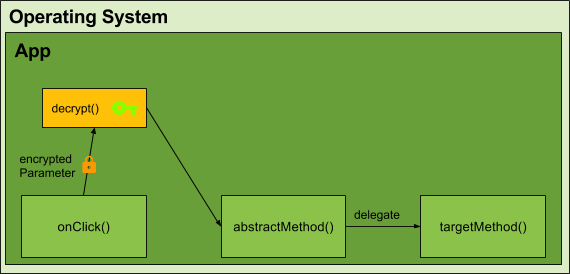
\includegraphics[width=0.8\textwidth]{data/encryptionAction.png}
    \caption{Encrypted actions to obfuscate dependencies}
    \label{fig:encryptionAction}
\end{figure}
